\documentclass[11pt,letterpaper]{article}
\usepackage[utf8]{inputenc}
\usepackage{caption} % for table captions
\usepackage{amsmath} % for multi-line equations and piecewises
\DeclareMathOperator{\sign}{sign}
\usepackage{graphicx}
\usepackage{relsize}
%\usepackage{textcomp}
\usepackage{xspace}
\usepackage{verbatim} % for block comments
%\usepackage{subfig} % for subfigures
\usepackage{enumitem} % for a) b) c) lists
\newcommand{\Cyclus}{\textsc{Cyclus}\xspace}%
\newcommand{\Cycamore}{\textsc{Cycamore}\xspace}%
\newcommand{\deploy}{\texttt{d3ploy}\xspace}%
\newcommand{\Deploy}{\texttt{D3ploy}\xspace}%
\usepackage{tabularx}
\usepackage{color}
\usepackage[acronym,toc]{glossaries}
\newacronym[longplural={metric tons of heavy metal}]{MTHM}{MTHM}{metric ton of heavy metal}
\newacronym{ABM}{ABM}{agent-based modeling}
\newacronym{ACDIS}{ACDIS}{Program in Arms Control \& Domestic and International Security}
\newacronym{AHTR}{AHTR}{Advanced High Temperature Reactor}
\newacronym{ANDRA}{ANDRA}{Agence Nationale pour la gestion des D\'echets RAdioactifs, the French National Agency for Radioactive Waste Management}
\newacronym{ANL}{ANL}{Argonne National Laboratory}
\newacronym{API}{API}{application programming interface}
\newacronym{ARCH}{ARCH}{autoregressive conditional heteroskedastic}
\newacronym{ARE}{ARE}{Aircraft Reactor Experiment}
\newacronym{ARFC}{ARFC}{Advanced Reactors and Fuel Cycles}
\newacronym{ARMA}{ARMA}{autoregressive moving average}
\newacronym{ASME}{ASME}{American Society of Mechanical Engineers}
\newacronym{ATWS}{ATWS}{Anticipated Transient Without Scram}
\newacronym{BDBE}{BDBE}{Beyond Design Basis Event}
\newacronym{BIDS}{BIDS}{Berkeley Institute for Data Science}
\newacronym{BOL}{BOL}{Beginning-of-Life}
\newacronym{BSD}{BSD}{Berkeley Software Distribution}
\newacronym{CAFCA}{CAFCA}{ Code for Advanced Fuel Cycles Assessment }
\newacronym{CASL}{CASL}{Consortium for Advanced Simulation of Light Water Reactors}
\newacronym{CDTN}{CDTN}{Centro de Desenvolvimento da Tecnologia Nuclear}
\newacronym{CEA}{CEA}{Commissariat \`a l'\'Energie Atomique et aux \'Energies Alternatives}
\newacronym{CI}{CI}{continuous integration}
\newacronym{CNEC}{CNEC}{Consortium for Nonproliferation Enabling Capabilities}
\newacronym{CNEN}{CNEN}{Comiss\~{a}o Nacional de Energia Nuclear}
\newacronym{CNERG}{CNERG}{Computational Nuclear Engineering Research Group}
\newacronym{COSI}{COSI}{Commelini-Sicard}
\newacronym{COTS}{COTS}{commercial, off-the-shelf}
\newacronym{CSNF}{CSNF}{commercial spent nuclear fuel}
\newacronym{CTAH}{CTAHs}{Coiled Tube Air Heaters}
\newacronym{CUBIT}{CUBIT}{CUBIT Geometry and Mesh Generation Toolkit}
\newacronym{CURIE}{CURIE}{Centralized Used Fuel Resource for Information Exchange}
\newacronym{DAG}{DAG}{directed acyclic graph}
\newacronym{DANESS}{DANESS}{Dynamic Analysis of Nuclear Energy System Strategies}
\newacronym{DBE}{DBE}{Design Basis Event}
\newacronym{DESAE}{DESAE}{Dynamic Analysis of Nuclear Energy Systems Strategies}
\newacronym{DHS}{DHS}{Department of Homeland Security}
\newacronym{DOE}{DOE}{Department of Energy}
\newacronym{DRACS}{DRACS}{Direct Reactor Auxiliary Cooling System}
\newacronym{DRE}{DRE}{dynamic resource exchange}
\newacronym{DSNF}{DSNF}{DOE spent nuclear fuel}
\newacronym{DYMOND}{DYMOND}{Dynamic Model of Nuclear Development }
\newacronym{EBS}{EBS}{Engineered Barrier System}
\newacronym{EDZ}{EDZ}{Excavation Disturbed Zone}
\newacronym{EIA}{EIA}{U.S. Energy Information Administration}
\newacronym{EPA}{EPA}{Environmental Protection Agency}
\newacronym{EP}{EP}{Engineering Physics}
\newacronym{FCO}{FCO}{Fuel Cycle Options}
\newacronym{FCT}{FCT}{Fuel Cycle Technology}
\newacronym{FCWMD}{FCWMD}{Fuel Cycle and Waste Management Division}
\newacronym{FEHM}{FEHM}{Finite Element Heat and Mass Transfer}
\newacronym{FEPs}{FEPs}{Features, Events, and Processes}
\newacronym{FHR}{FHR}{Fluoride-Salt-Cooled High-Temperature Reactor}
\newacronym{FLiBe}{FLiBe}{Fluoride-Lithium-Beryllium}
\newacronym{GCAM}{GCAM}{Global Change Assessment Model}
\newacronym{GDSE}{GDSE}{Generic Disposal System Environment}
\newacronym{GDSM}{GDSM}{Generic Disposal System Model}
\newacronym{GENIUSv1}{GENIUSv1}{Global Evaluation of Nuclear Infrastructure Utilization Scenarios, Version 1}
\newacronym{GENIUSv2}{GENIUSv2}{Global Evaluation of Nuclear Infrastructure Utilization Scenarios, Version 2}
\newacronym{GENIUS}{GENIUS}{Global Evaluation of Nuclear Infrastructure Utilization Scenarios}
\newacronym{GPAM}{GPAM}{Generic Performance Assessment Model}
\newacronym{GRSAC}{GRSAC}{Graphite Reactor Severe Accident Code}
\newacronym{GUI}{GUI}{graphical user interface}
\newacronym{HLW}{HLW}{high level waste}
\newacronym{HPC}{HPC}{high-performance computing}
\newacronym{HTC}{HTC}{high-throughput computing}
\newacronym{HTGR}{HTGR}{High Temperature Gas-Cooled Reactor}
\newacronym{IAEA}{IAEA}{International Atomic Energy Agency}
\newacronym{IEMA}{IEMA}{Illinois Emergency Mangament Agency}
\newacronym{INL}{INL}{Idaho National Laboratory}
\newacronym{IPRR1}{IRP-R1}{Instituto de Pesquisas Radioativas Reator 1}
\newacronym{IRP}{IRP}{Integrated Research Project}
\newacronym{ISFSI}{ISFSI}{Independent Spent Fuel Storage Installation}
\newacronym{ISRG}{ISRG}{Independent Student Research Group}
\newacronym{JFNK}{JFNK}{Jacobian-Free Newton Krylov}
\newacronym{LANL}{LANL}{Los Alamos National Laboratory}
\newacronym{LBNL}{LBNL}{Lawrence Berkeley National Laboratory}
\newacronym{LCOE}{LCOE}{levelized cost of electricity}
\newacronym{LDRD}{LDRD}{laboratory directed research and development}
\newacronym{LFR}{LFR}{Lead-Cooled Fast Reactor}
\newacronym{LGPL}{LGPL}{Lesser GNU Public License}
\newacronym{LLNL}{LLNL}{Lawrence Livermore National Laboratory}
\newacronym{LMFBR}{LMFBR}{Liquid-Metal-cooled Fast Breeder Reactor}
\newacronym{LOFC}{LOFC}{Loss of Forced Cooling}
\newacronym{LOHS}{LOHS}{Loss of Heat Sink}
\newacronym{LOLA}{LOLA}{Loss of Large Area}
\newacronym{LP}{LP}{linear program}
\newacronym{LWR}{LWR}{Light Water Reactor}
\newacronym{MARKAL}{MARKAL}{MARKet and ALlocation}
\newacronym{MA}{MA}{minor actinide}
\newacronym{MCNP}{MCNP}{Monte Carlo N-Particle code}
\newacronym{MILP}{MILP}{mixed-integer linear program}
\newacronym{MIT}{MIT}{the Massachusetts Institute of Technology}
\newacronym{MOAB}{MOAB}{Mesh-Oriented datABase}
\newacronym{MOOSE}{MOOSE}{Multiphysics Object-Oriented Simulation Environment}
\newacronym{MOX}{MOX}{mixed oxide}
\newacronym{MSBR}{MSBR}{Molten Salt Breeder Reactor}
\newacronym{MSRE}{MSRE}{Molten Salt Reactor Experiment}
\newacronym{MSR}{MSR}{Molten Salt Reactor}
\newacronym{NAGRA}{NAGRA}{National Cooperative for the Disposal of Radioactive Waste}
\newacronym{NCSA}{NCSA}{National Center for Supercomputing Applications}
\newacronym{NEAMS}{NEAMS}{Nuclear Engineering Advanced Modeling and Simulation}
\newacronym{NEUP}{NEUP}{Nuclear Energy University Programs}
\newacronym{NFCSim}{NFCSim}{Nuclear Fuel Cycle Simulator}
\newacronym{NFC}{NFC}{Nuclear Fuel Cycle}
\newacronym{NGNP}{NGNP}{Next Generation Nuclear Plant}
\newacronym{NMWPC}{NMWPC}{Nuclear MW Per Capita}
\newacronym{NNSA}{NNSA}{National Nuclear Security Administration}
\newacronym{NPRE}{NPRE}{Department of Nuclear, Plasma, and Radiological Engineering}
\newacronym{NQA1}{NQA-1}{Nuclear Quality Assurance - 1}
\newacronym{NRC}{NRC}{Nuclear Regulatory Commission}
\newacronym{NSF}{NSF}{National Science Foundation}
\newacronym{NSSC}{NSSC}{Nuclear Science and Security Consortium}
\newacronym{NUWASTE}{NUWASTE}{Nuclear Waste Assessment System for Technical Evaluation}
\newacronym{NWF}{NWF}{Nuclear Waste Fund}
\newacronym{NWTRB}{NWTRB}{Nuclear Waste Technical Review Board}
\newacronym{OCRWM}{OCRWM}{Office of Civilian Radioactive Waste Management}
\newacronym{ORION}{ORION}{ORION}
\newacronym{ORNL}{ORNL}{Oak Ridge National Laboratory}
\newacronym{PARCS}{PARCS}{Purdue Advanced Reactor Core Simulator}
\newacronym{PBAHTR}{PB-AHTR}{Pebble Bed Advanced High Temperature Reactor}
\newacronym{PBFHR}{PB-FHR}{Pebble-Bed Fluoride-Salt-Cooled High-Temperature Reactor}
\newacronym{PEI}{PEI}{Peak Environmental Impact}
\newacronym{PH}{PRONGHORN}{PRONGHORN}
\newacronym{PI}{PI}{Principal Investigator}
\newacronym{PNNL}{PNNL}{Pacific Northwest National Laboratory}
\newacronym{PRIS}{PRIS}{Power Reactor Information System}
\newacronym{PRKE}{PRKE}{Point Reactor Kinetics Equations}
\newacronym{PSPG}{PSPG}{Pressure-Stabilizing/Petrov-Galerkin}
\newacronym{PWAR}{PWAR}{Pratt and Whitney Aircraft Reactor}
\newacronym{PWR}{PWR}{Pressurized Water Reactor}
\newacronym{PyNE}{PyNE}{Python toolkit for Nuclear Engineering}
\newacronym{PyRK}{PyRK}{Python for Reactor Kinetics}
\newacronym{QA}{QA}{quality assurance}
\newacronym{RDD}{RD\&D}{Research Development and Demonstration}
\newacronym{RD}{R\&D}{Research and Development}
\newacronym{RELAP}{RELAP}{Reactor Excursion and Leak Analysis Program}
\newacronym{RIA}{RIA}{Reactivity Insertion Accident}
\newacronym{RIF}{RIF}{Region-Institution-Facility}
\newacronym{SAM}{SAM}{Simulation and Modeling}
\newacronym{SCF}{SCF}{Software Carpentry Foundation}
\newacronym{SFR}{SFR}{Sodium-Cooled Fast Reactor}
\newacronym{SINDAG}{SINDA{\textbackslash}G}{Systems Improved Numerical Differencing Analyzer $\backslash$ Gaski}
\newacronym{SKB}{SKB}{Svensk K\"{a}rnbr\"{a}nslehantering AB}
\newacronym{SNF}{SNF}{spent nuclear fuel}
\newacronym{SNL}{SNL}{Sandia National Laboratory}
\newacronym{SNM}{SNM}{Special Nuclear Material}
\newacronym{STC}{STC}{specific temperature change}
\newacronym{SUPG}{SUPG}{Streamline-Upwind/Petrov-Galerkin}
\newacronym{SWF}{SWF}{Separations and Waste Forms}
\newacronym{SWU}{SWU}{Separative Work Unit}
\newacronym{SandO}{S\&O}{Signatures and Observables}
\newacronym{THW}{THW}{The Hacker Within}
\newacronym{TRIGA}{TRIGA}{Training Research Isotope General Atomic}
\newacronym{TRISO}{TRISO}{Tristructural Isotropic}
\newacronym{TSM}{TSM}{Total System Model}
\newacronym{TSPA}{TSPA}{Total System Performance Assessment for the Yucca Mountain License Application}
\newacronym{UDB}{UDB}{Unified Database}
\newacronym{UFD}{UFD}{Used Fuel Disposition}
\newacronym{UML}{UML}{Unified Modeling Language}
\newacronym{UNFSTANDARDS}{UNFST\&DARDS}{Used Nuclear Fuel Storage, Transportation \& Disposal Analysis Resource and Data System}
\newacronym{UOX}{UOX}{uranium oxide}
\newacronym{UQ}{UQ}{uncertainty quantification}
\newacronym{US}{US}{United States}
\newacronym{UW}{UW}{University of Wisconsin}
\newacronym{VISION}{VISION}{the Verifiable Fuel Cycle Simulation Model}
\newacronym{VV}{V\&V}{verification and validation}
\newacronym{WIPP}{WIPP}{Waste Isolation Pilot Plant}
\newacronym{YMG}{YMG}{Young Members Group}
\newacronym{YMR}{YMR}{Yucca Mountain Repository Site}
\newacronym{NEI}{NEI}{Nuclear Energy Institute}
%\newacronym{<++>}{<++>}{<++>}
%\newacronym{<++>}{<++>}{<++>}

\definecolor{bg}{rgb}{0.95,0.95,0.95}
\newcolumntype{b}{X}
\newcolumntype{f}{>{\hsize=.15\hsize}X}
\newcolumntype{s}{>{\hsize=.5\hsize}X}
\newcolumntype{m}{>{\hsize=.75\hsize}X}
\newcolumntype{r}{>{\hsize=1.1\hsize}X}
\usepackage{titling}
\usepackage[hang,flushmargin]{footmisc}
\renewcommand*\footnoterule{}
\usepackage{tikz}


\usetikzlibrary{shapes.geometric,arrows}
\tikzstyle{process} = [rectangle, rounded corners, 
minimum width=1cm, minimum height=1cm,text centered, draw=black, 
fill=blue!30]
\tikzstyle{arrow} = [thick,->,>=stealth]


\graphicspath{{figures/}}
\title{DDCA GLOBAL}
\author{Gwendolyn J. Chee, Roberto E. Fairhurst, 
\\ \vspace{0.5em} Robert R. Flanagan, Kathryn D. Huff}


\begin{document}
	\begin{titlepage}
	\maketitle
	\thispagestyle{empty}
	\end{titlepage}

%----------------------------------------------------------------%
\section{Introduction}
\gls{NFC} simulation scenarios are constrained objective functions. 
The objectives are systemic demands such as "1\% power growth", 
while an example of a constraint is the availability of new nuclear 
technology. 
To add ease in setting up nuclear fuel cycle simulations, \gls{NFC}
simulators should bring demand responsive deployment decisions into 
the dynamics of the simulation logic \cite{huff_current_2017}. 
While automated power production deployment is common in most fuel 
cycle simulators, automated deployment of supportive fuel cycle 
facilities is non-existent. 

Instead, the user must detail the deployment timeline of all 
supporting facilities or have infinite capacity support facilities. 
Thus, a next generation \gls{NFC} simulator should predictively and 
automatically deploy fuel cycle facilities to meet user defined 
power demand. 
This report discusses demonstration of a new solution, 
\texttt{d3ploy}, enabling demand driven deployment in \Cyclus. 

\Cyclus is an agent-based nuclear fuel cycle simulation framework 
\cite{huff_fundamental_2016}. 
Each entity (i.e. Region, Institution, or Facility) in the fuel 
cycle is modeled as an agent. 
Institution agents
are responsible for deploying and decommissioning facility agents 
and can represent a legal operating organization such as a 
utility, government, etc \cite{huff_fundamental_2016}. 

The Demand-Driven \Cycamore Archetypes project (NEUP-FY16-10512) 
aims to develop \Cyclus's demand-driven deployment capabilities. 
This capability is developed in the form of a \Cyclus Institution
agent that deploys facilities to meet the front-end and back-end 
fuel cycle demands based on a user-defined commodity demand. 
Its goal is to meet supply for any commodity while minimizing 
undersupply.
This demand-driven deployment capability is referred to as 
\deploy. 

In this report, we will explain the capabilities of \deploy, 
demonstrate how \deploy can be used in a flat power transition 
to meet the primary objective of minimizing undersupply of all 
commodities in the simulation. 
The goal is to study a basic flat power demand scenario 
and provide recommendations and insights to inform 
decisions about parameter inputs when setting up 
larger flat power demand transition scenarios that include many 
facilities. 

\section{D3ploy capabilities}
\subsection{Core Capability of \deploy}
At each time step, \deploy predicts demand and supply of each 
commodity for the next time step.
Then, \deploy deploys facilities to meet predicted demand. 
\Deploy's primary objective is to minimize the number of time 
steps of undersupply of any commodity. 

When there is a predicted undersupply of a commodity, \deploy looks 
at what facilities it has that provides that commodity and 
will deploy the fewest number of facilities
to meet the predicted undersupply. 
This logic is available in \texttt{solver.py}. 

\subsection{Basic User-Defined Input Variables}
The user is able to input specific variables to customize their
simulation. 
Descriptions of each input variable can be found in the 
readme of the repository [https://github.com/arfc/d3ploy]. 

Essentially, the user must define the facilities they want the 
institution to control and their corresponding capacities. 
The user must also define the driving commodity, its demand 
equation and what method they want the institution to predict 
demand and supply with. 

They also have the option to give an equation that governs
preference for that facility compared to other facilities that 
provide the same commodity. 
The user also has an option to constrain deployment of a facility 
until there is a accumulation of the inventory of a specific commodity.  
The user can also define an initial facility list of facilities that 
are present in the institution at the beginning of the simulation. 

\subsection{Prediction Algorithms}
Three interchangeable algorithm types govern demand and supply 
predictions: non-optimizing, deterministic optimizing and stochastic
optimizing. 

There are three methods implemented for the non-optimizing model: 
Autoregressive moving average (ARMA), autoregressive 
conditional heteroskedasticity (ARCH).
There are four methods implemented for the deterministic optimizing model: 
Polynomial fit regression, simple exponential smoothing,  
triple exponential smoothing (holt-winters) and fast fourier 
transform (fft). 
There is one method implemented for stochastic optimizing model: 
stepwise seasonal.  

The user can choose which prediction algorithm governs each specific 
\deploy facility. 

\subsection{Difference between Demand and Supply Driven Institutions}
Within \deploy, there are two institutions: 
\texttt{DemandDrivenDeploymentInst} and \texttt{SupplyDrivenDeploymentInst}. 
The prior is used for the front-end of the fuel cycle and the latter is used 
for the back-end. 
Front-end facilities are facilities that exist before the reactor 
in a nuclear fuel cycle such as a fuel fabrication facility etc. 
Back-end facilities are facilities that exist after the reactor in a nuclear 
fuel cycle, such as a reprocessing facility etc. 
The reason for this separation is to let facilities have the choice 
to demand for supply or demand for capacity. 
For example, in the front end facilities, the reactor has a demand for 
fuel, using \texttt{DemandDrivenDeploymentInst}, it triggers the fuel 
fabrication facility to deploy facilities to create supply to meet 
the demand. 
Whereas, for the back end facilities, the reactor generates spent fuel 
, there is a demand for waste repository facility to accept the 
spent fuel, using \texttt{SupplyDrivenDeploymentInst}, it triggers the
deployment of a waste repository to create a capacity for spent fuel 
to meet the available supply. 

\subsection{Installed Capacity}
The user can choose between deploying facilities based on the difference 
between predicted demand and predicted supply or predicted demand and 
installed capacity. 
There are two reasons for wanting to use installed capacity over predicted 
supply. 
The first is for facilities that provide intermittent supply, such as a 
reactor facility that has a designated refueling time. 
During time steps where a reactor is refueling, the user might not 
want \deploy to deploy more facilities to make up for the lack of supply
caused by this one time step gap in supply. 
The second is for situations where the input commodity for a facility has
run out in a simulation and the facility that produces the input commodity 
is no longer commissionable. 
Therefore, with the demand for the output commodity of that facility, \deploy
would deploy that facility to meet the demand, however due to the lack of 
the input commodity, even if there are infinite numbers of that facility, 
it will not produce the output commodity. 
For example, in a transition scenario to fast reactors that require plutonium 
from \gls{LWR}'s \gls{SNF}, if the fast reactor's demand for plutonium exceeds
the inventory provided by \gls{LWR}s before they were decommissioned, it will 
result in the deployment of mixer facilities that generate the fast reactor 
fuel despite the lack of plutonium to generate the fuel. 
This is an example of a poorly set up transition scenario. 

\subsection{Supply/Capacity Buffer}
In \texttt{DemandDrivenDeploymentInst}, the user can choose to provide a
buffer for the predicted supply so that \deploy will ensure that the predicted 
supply will meet the predicted demand with the additional buffer. 

In \texttt{SupplyDrivenDeploymentInst}, the user can choose to provide a
buffer for the predicted capacity so that \deploy will ensure predicted 
capacity meets the predicted supply with the additional buffer. 
The buffer can be defined as a percentage value or an absolute value.  

\section{Methods for demonstration of d3ploy capabilities}
A flat power simulation is set up to demonstrate \deploy's 
capabilities. 
A balance between the various system parameters must be 
met for each type of simulation to ideally meet the goal of 
minimizing undersupply and under capacity for the various 
commodities. 

This simulation is a basic transition scenario that only includes three 
types of facilities: \texttt{source}, \texttt{reactor} and \texttt{sink}.
The reason for setting up a basic flat power demand scenario is to 
inform decisions about parameter inputs when setting up larger flat power 
demand transition scenarios that include many facilities. 

\subsection{Transition Scenario: Flat Demand}
In this section, a flat power transition scenario is studied and 
recommendations and insights on specific parameters are 
discussed. 
Table \ref{tab:transition-scenario-flat-power} shows the parameters 
used for this transition scenario. 
The input file used to generate this simulation can be found in

\noindent
$/d3ploy/input/constant\_transition.xml$ and the file used 
to run the simulation and generate the plots can be found in 

\noindent
$/d3ploy/tests/performance\_tests/algorithm\_performance\_tests\_constant$
\linebreak
$\_transition.py$

The ten initial reactors in the simulation have different cycle 
lengths so that they refuel at different times. 
In figure \ref{fig:flattransition-power}, there are two time steps
where supply falls under demand, this is due to the combined 
refueling of multiple \texttt{new reactors}. 
By setting the supply buffer to 3000MW (the capacity of 3 reactors), 
the user is able to minimize the number of time steps where there 
is an undersupply. 
It is important to perform a small sensitivity analysis of the size 
of buffer to use for each commodity to ensure that there is no 
undersupply based on the nuances of the facility type: 
refueling in a reactor etc. 
If the \texttt{new reactors} were configured such that they had 
no refueling, there will be no time steps where supply falls under 
demand.
This is shown in figure \ref{fig:flattransition-power-norefuel}, 
however, a reactor without refueling is unrealistic. 
Future work should allow for randomization of reactor cycle length 
so that refueling occurs at different times when the same reactor 
facility type is deployed to avoid the issue where all the same 
reactors that were deployed at the same time step having to refuel 
at the same time. 

Figure \ref{fig:flattransition-fuel} shows the demand and supply 
for fuel in the simulation. 
An initial facility with a large capacity of fuel is initially
deployed to meet the large initial fuel demand for the starting
up of ten reactors. 
There are no time steps where there is an undersupply. 
I suggest that for future simulations where a facility requires a
large amount of start up commodity such as in this simulation 
where ten reactors start up at the same time, and thus require 
a large amount of start up fuel. 
The user should add an initial facility with a large throughput
to exist for the first few time steps in the simulation, so as 
to prevent \deploy from deploying a large amount of supporting
facilities that end up being redundant at the later parts of 
the simulation. 
This could also be circumvented by introducing decommissioning 
capability into \deploy.  

\begin{table}[!htbp]
	\centering
	\caption {Transition Scenario Flat Demand Parameters}
	\label{tab:transition-scenario-flat-power}
	\begin{tabular}{|l|p{6.5cm}|}
		\hline
		\textbf{Parameter} & \\
		\hline
		\textbf{Facilities Present} & \texttt{Source} (Capacity: 3000kg), \texttt{Reactor} (Capacity: 1000MW), \texttt{Sink} \\
		\hline
		\textbf{New Reactor Parameters} & Cycle time: 18, Refuel time: 1\\
		\hline
		\textbf{Driving Commodity} & \texttt{Power}\\
		\hline
		\textbf{Demand Equation} & 10000 MW \\
		\hline
		\textbf{Supply Buffer} & 3000 MW (3 reactor capacities)\\
		\hline
	\end{tabular}
\end{table}

\begin{figure}[!htbp]
	\begin{center}
		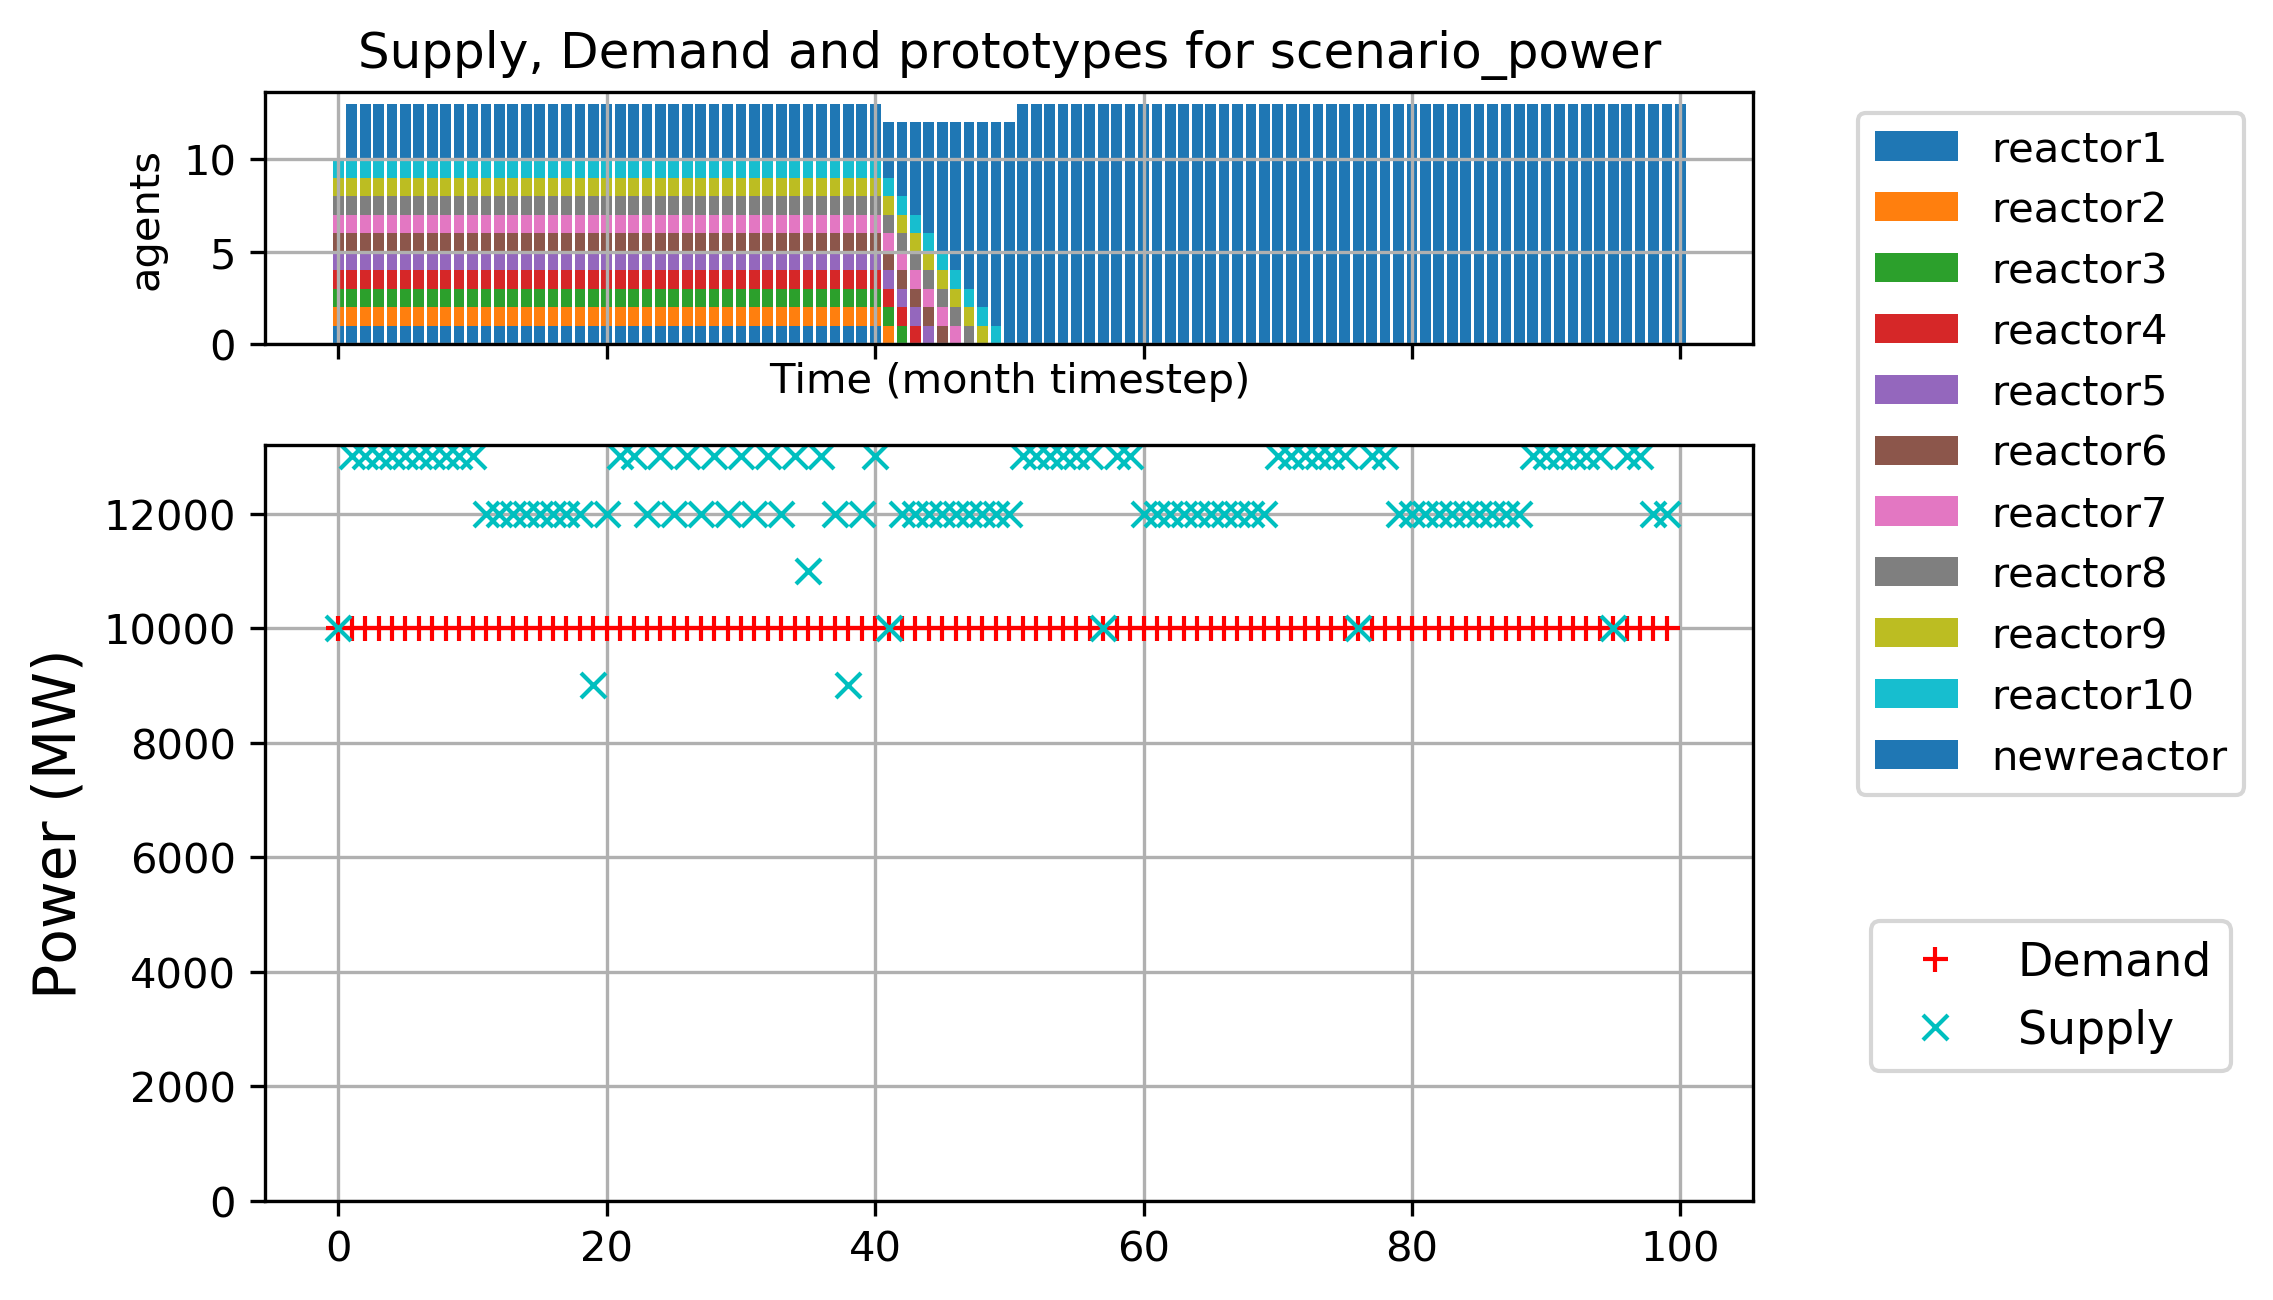
\includegraphics[scale=0.65]{figures/flattransition-power.png}
	\end{center}
        \caption{Power demand and supply plot for a flat power demand transition scenario where new reactor has cycle length = 20, refueling length time = 1}
	\label{fig:flattransition-power}
\end{figure}

\begin{figure}[!htbp]
	\begin{center}
		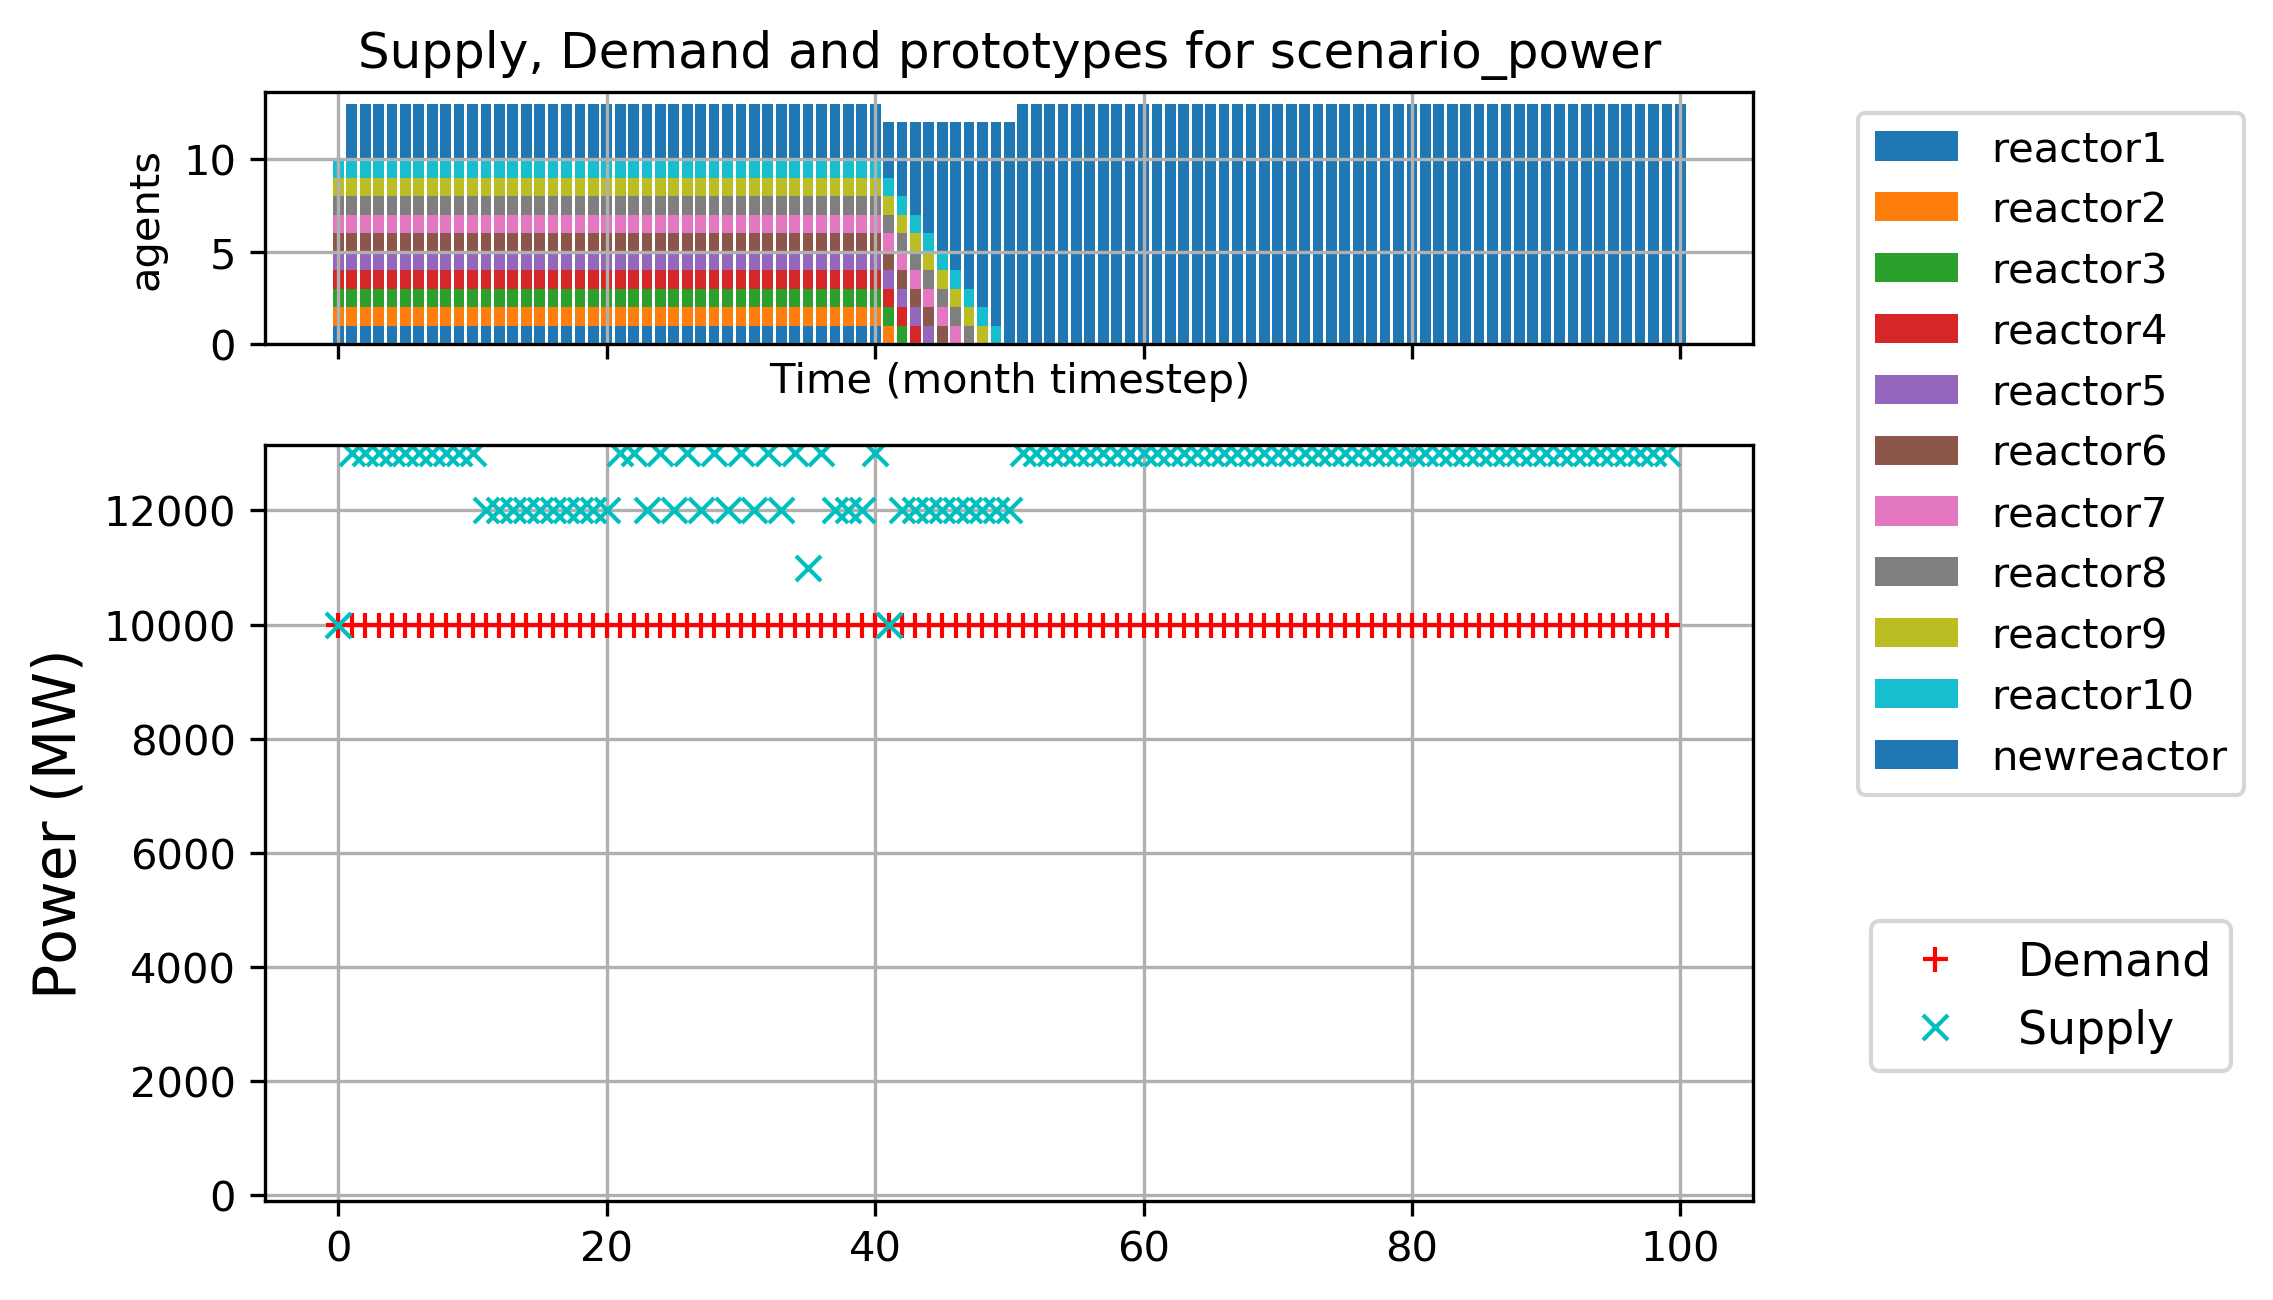
\includegraphics[scale=0.65]{figures/flattransition-power-norefuel.png}
	\end{center}
        \caption{Power demand and supply plot for a flat power demand transition scenario where new reactor has cycle length = 20, refueling length time = 0}
	\label{fig:flattransition-power-norefuel}
\end{figure}

\begin{figure}[!htbp]
	\begin{center}
		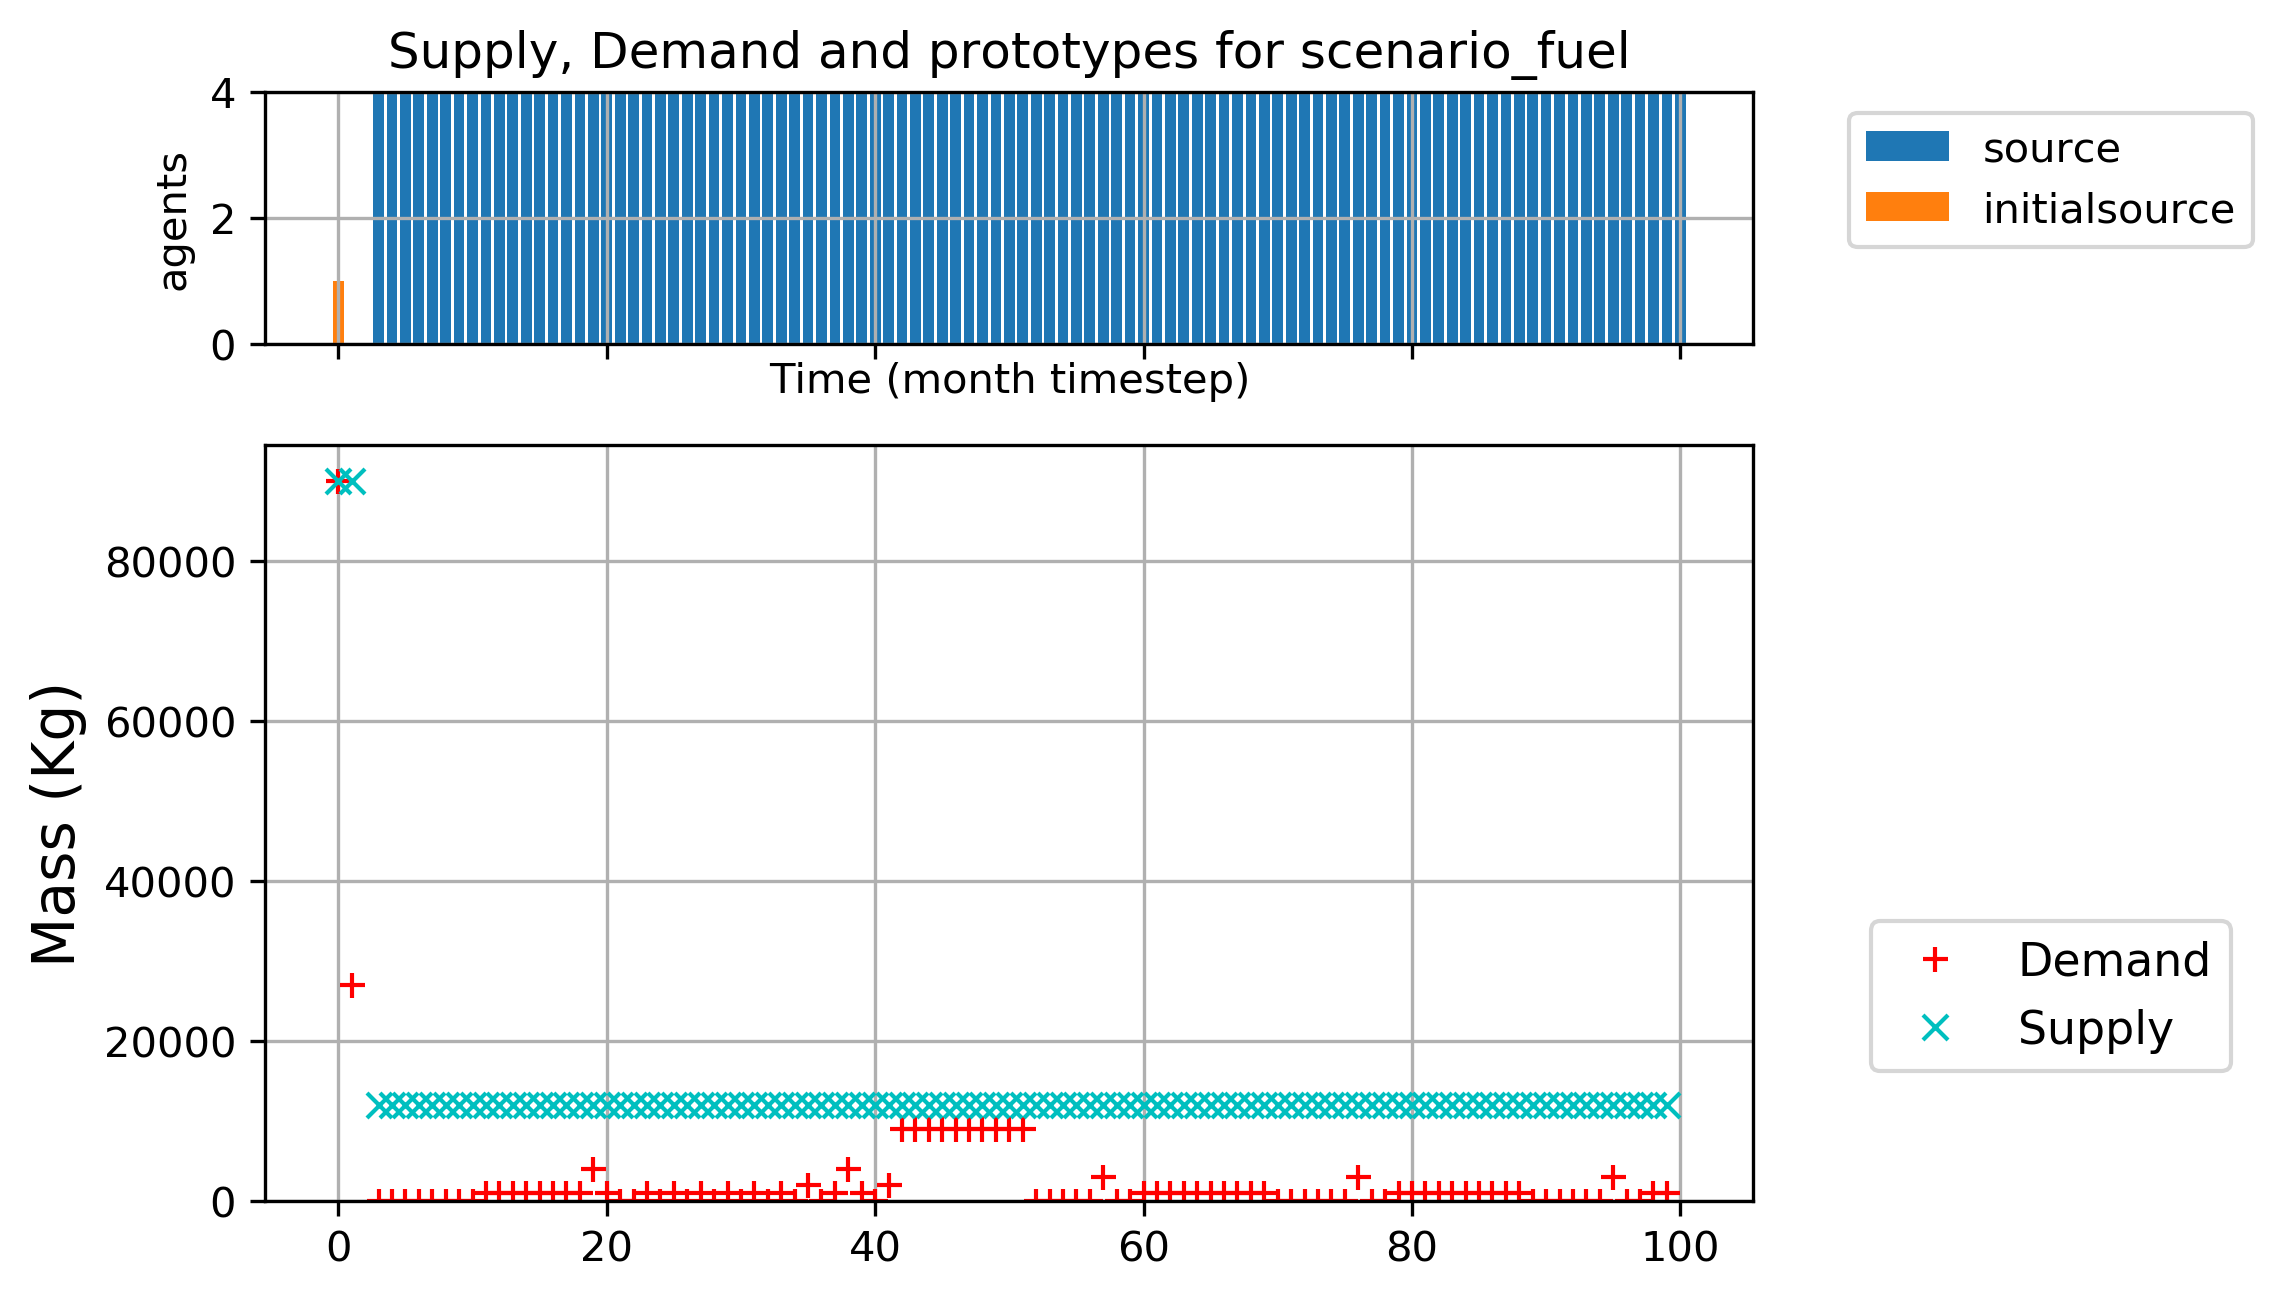
\includegraphics[scale=0.65]{figures/flattransition-fuel.png}
	\end{center}
        \caption{Fuel demand and supply plot for a flat power demand transition scenario where new reactor has cycle length = 20, refueling length time = 1}
	\label{fig:flattransition-fuel}
\end{figure}

\pagebreak
\section{Conclusion}
This report describes the capabilities of \deploy, demonstrates 
the use of \deploy in a basic flat power transition scenario and 
provides insights on parameter inputs when setting up larger flat 
power demand transition scenarios that include many facilities. 

\section{Acknowledgements}
This research is funded by the \gls{DOE} Office of 
Nuclear Energy's Nuclear Energy University Program (Project 16-10512) 
"Demand-Driven Cycamore Archetypes". The authors want to thank 
members of the \gls{ARFC} group at the University of Illinois at 
Urbana-Champaign. 
We also thank our colleagues from the \Cyclus community, 
particularly those in the University of Wisconsin 
\gls{CNERG} and the University of South Carolina Energy Research 
Group (ERGS) for collaborative \Cyclus development.
%----------------------------------------------------------------%

\pagebreak 
\bibliographystyle{plain}
\bibliography{bibliography}

\end{document}


